\documentclass[conference]{IEEEtran}

% Packages for graphics, math, and bibliography
\usepackage{graphicx}
\usepackage{amsmath}
\usepackage{cite}

\usepackage{tabularx}

% Title and author information
\title{Your Thesis Title}
\author{Your Name}
\date{\today}

\begin{document}
	
	\maketitle
	\begin{abstract}
		This is the abstract of your paper. It provides a concise summary of the paper's key aspects, such as the problem statement, methodology, and main results. The abstract should be informative and enticing to the readers, providing a glimpse into the contents of the paper.
	\end{abstract}
	
	\section{Introduction}
	% Your introduction goes here
	Lorem ipsum dolor sit amet, consectetur adipiscing elit, sed do eiusmod tempor incididunt ut labore et dolore magna aliqua. Ut enim ad minim veniam, quis nostrud exercitation ullamco laboris nisi ut aliquip ex ea commodo consequat. Duis aute irure dolor in reprehenderit in voluptate velit esse cillum dolore eu fugiat nulla pariatur. Excepteur sint occaecat cupidatat non proident, sunt in culpa qui officia deserunt mollit anim id est laborum
	
	\section{Related Work}
	% Literature review and related work analysis
	Lorem ipsum dolor sit amet, consectetur adipiscing elit, sed do eiusmod tempor incididunt ut labore et dolore magna aliqua. Ut enim ad minim veniam, quis nostrud exercitation ullamco laboris nisi ut aliquip ex ea commodo consequat. Duis aute irure dolor in reprehenderit in voluptate velit esse cillum dolore eu fugiat nulla pariatur. Excepteur sint occaecat cupidatat non proident, sunt in culpa qui officia deserunt mollit anim id est laborum.
	
	Really, attention is all you need  \cite{vaswani2017attention}
	
\begin{table}[htbp]
	\centering
	\caption{Sample Table in IEEE Style}
	\label{tab:sample}
	\begin{tabularx}{\columnwidth}{|X|X|X|}
		\hline
		\textbf{Column 1} & \textbf{Column 2} & \textbf{Column 3} \\
		\hline
		Data 1 & Data 2 & Data 3 \\
		\hline
		Data 4 & Data 5 & Data 6 \\
		\hline
	\end{tabularx}
\end{table}
	
	\section{Methodology}
	% Explain your research methodology and approach
	Lorem ipsum dolor sit amet, consectetur adipiscing elit, sed do eiusmod tempor incididunt ut labore et dolore magna aliqua. Ut enim ad minim veniam, quis nostrud exercitation ullamco laboris nisi ut aliquip ex ea commodo consequat. Duis aute irure dolor in reprehenderit in voluptate velit esse cillum dolore eu fugiat nulla pariatur. Excepteur sint occaecat cupidatat non proident, sunt in culpa qui officia deserunt mollit anim id est laborum.
	
	\cite{russell2021human}
	
		% Example equation
	\begin{equation}
		\label{eq:example}
		F(x) = \int_{a}^{b} f(x) \, dx
	\end{equation}
	
	\section{Results}
	% Present your research findings and results
	Lorem ipsum dolor sit amet, consectetur adipiscing elit, sed do eiusmod tempor incididunt ut labore et dolore magna aliqua. Ut enim ad minim veniam, quis nostrud exercitation ullamco laboris nisi ut aliquip ex ea commodo consequat. Duis aute irure dolor in reprehenderit in voluptate velit esse cillum dolore eu fugiat nulla pariatur. Excepteur sint occaecat cupidatat non proident, sunt in culpa qui officia deserunt mollit anim id est laborum
		
	In Equation~\ref{eq:example}, $f(x)$ represents the input function and $F(x)$ is the result of its integration.
		% Example figure
	\begin{figure}[htbp]
		\centering
		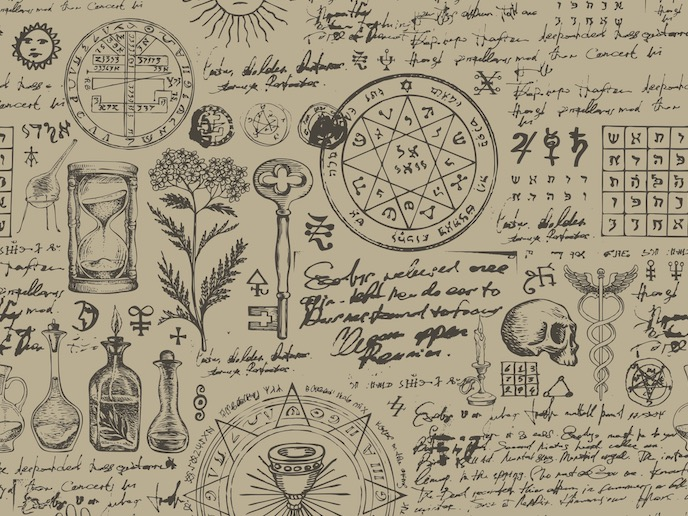
\includegraphics[width=0.8\columnwidth]{image}
		\caption{Example figure}
		\label{fig:example}
	\end{figure}
	
	\section{Discussion}
	% Analyze and discuss the implications of your results
	Lorem ipsum dolor sit amet, consectetur adipiscing elit, sed do eiusmod tempor incididunt ut labore et dolore magna aliqua. 
		Figure~\ref{fig:example} illustrates an example figure included in your thesis.
		
	\section{Conclusion}
	% Summarize your thesis and highlight the key contributions
	Lorem ipsum dolor sit amet, consectetur adipiscing elit, sed do eiusmod tempor incididunt ut labore et dolore magna aliqua. Ut enim ad minim veniam, quis nostrud exercitation ullamco laboris nisi ut aliquip ex ea commodo consequat. Duis aute irure dolor in reprehenderit in voluptate velit esse cillum dolore eu fugiat nulla pariatur. Excepteur sint occaecat cupidatat non proident, sunt in culpa qui officia deserunt mollit anim id est laborum
	
	
	% Bibliography
	\bibliographystyle{IEEEtran}
	\bibliography{references.bib}
	
\end{document}
